\documentclass[12pt,a4paper]{article}
\usepackage[utf8]{inputenc}
\usepackage[T1]{fontenc}
\usepackage[portuguese]{babel}
\usepackage{amsmath,amssymb}
\usepackage{graphicx}
% Caminho padrão para figuras (permite usar apenas o nome do arquivo nas inclusões)
\graphicspath{{Arquivos/Q3/results/figures/}}
\usepackage{geometry}
\usepackage{hyperref}
\usepackage{caption}
\usepackage{float}
\usepackage{longtable}
\usepackage{booktabs}
\usepackage{listings}
\usepackage{enumitem}
\usepackage{xcolor}
\usepackage{colortbl}
\geometry{a4paper, margin=1in}

\lstset{
  basicstyle=\small\ttfamily,
  breaklines=true,
  frame=single,
  numbers=left,
  numberstyle=\tiny\color{gray},
  keywordstyle=\color{blue},
  commentstyle=\color{green!40!black},
  stringstyle=\color{purple},
  showstringspaces=false,
}

% Definição de linguagem para Assembly (RISC-V) no listings
\lstdefinelanguage{Assembly}{
    morekeywords={.text,.data,.globl,li,la,addi,add,sub,mul,div,rem,
        slli,srli,srai,andi,ori,xori,andi,or,xor,slt,slti,beq,bne,blt,bge,bgt,
        j,jal,jalr,ret,ecall,lw,sw,lb,lh,lb,sb,flw,fsw,fmv.d,fcvt.d.w,fmul.d,fadd.d,fsub.d,fdiv.d,
        fsd,fld,csrr,csrw,mv,lui,auipc},
    sensitive=true,
    morecomment=[l]{#},
}

\hypersetup{
  colorlinks=true,
  linkcolor=black,
  urlcolor=blue,
  pdftitle={Laboratório 1 - Assembly RISC-V},
  pdfauthor={Grupo}
}

\begin{document}

% -----------------------------
% capa (estilo semelhante ao OAC_LAB1)
% -----------------------------
\begin{titlepage}
    \begin{center}
        \vspace*{1cm}
        \includegraphics[width=5cm]{Lab_1/Logo_UnB.png}\\[1cm]

        {\LARGE \textbf{Universidade de Brasília}}\\[4pt]
        {\large Departamento de Ciência da Computação}\\[12pt]
        {\Large \textbf{Disciplina: CIC0099 -- Organização e Arquitetura de Computadores -- Unificado}}\\[20pt]

        {\huge \textbf{Laboratório 1}}\\[6pt]
        {\Large \textbf{Assembly RISC-V}}\\[2cm]

        \textbf{Grupo:} \\[4pt]
        \begin{tabular}{l}
            
            Gabriel de Sousa -- 211056000 \\
            Ana Luísa Reis Nascente -- 211045688 \\
            Guilherme Henrique Oliveira Araujo -- (matrícula) \\
            Gabriel Pinto Rodrigues -- 241002331 \\
            Victor Yan Martinez -- 241032994 \\
            
        \end{tabular}

        \vfill

        

        \vspace{0.8cm}
        \today
    \end{center}
\end{titlepage}

\pagenumbering{roman}
\tableofcontents
\newpage

\pagenumbering{arabic}

% -----------------------------
% introducao (estilo do relatório)
% -----------------------------
\section*{Introdução}
\addcontentsline{toc}{section}{Introdução}

Este relatório segue a estrutura solicitada no enunciado do Laboratório 1 (OAC\_LAB1). O objetivo principal é desenvolver habilidades práticas em linguagem Assembly RISC-V utilizando o simulador RARS e ferramentas de compilação cruzada. As atividades envolvem: implementação e análise de algoritmos em Assembly, medição de desempenho usando CSRs, comparação do código gerado pelo compilador cruzado gcc com diferentes níveis de otimização, e implementação da Transformada Discreta de Fourier (DFT) em Assembly.

O relatório está organizado na forma de \emph{resposta ao item}, contendo apenas os itens que valem ponto, e mantendo as perguntas explicitamente conforme solicitado no enunciado. As seções seguintes reproduzem as perguntas do enunciado para que as respostas possam ser inseridas diretamente abaixo de cada item.

% -----------------------------
% SEÇÃO 1 - RARS
% -----------------------------
\section*{(2.5) 1) Simulador/Montador RARS}
\addcontentsline{toc}{section}{1) Simulador/Montador RARS}

\subsection*{(2.5) 1.2) Considere a execução deste algoritmo em um processador RISC-V com frequência de clock de 50MHz que necessita 1 ciclo de clock para a execução de cada instrução $(CPI=1)$.}
Para os vetores de entrada de $n$ elementos já ordenados $V_{o}[n]=\{1,2,3,4,...,n\}$ e ordenados inversamente $V_{i}[n]=\{n,n-1,n-2,...,2,1\}$:

\begin{enumerate}
    \item[(1.5) a)] Para o procedimento \texttt{sort}, escreva as equações dos tempos de execução, $t_{o}(n)$ e $t_{i}(n)$, em função de $n$.
    \item[(1.0) b)] Para $n=\{10,20,30,40,50,60,70,80,90,100\}$, plote (em escala!) as duas curvas, $t_{o}(n)$ e $t_{i}(n)$, em um mesmo gráfico $n \times t$. Comente os resultados obtidos.
\end{enumerate}


\subsection*{1.2(a) Equações do Tempo de Execução}

As equações teóricas para o tempo de execução do algoritmo \texttt{SORT} foram desenvolvidas para o melhor caso (vetor já ordenado) e o pior caso (vetor ordenado de forma inversa), considerando um processador RISC-V com frequência de 50 MHz e CPI=1.

\subsubsection*{Caso Melhor (vetor já ordenado $V_{o}[n]=\{1,2,3,...,n\}$)}
\begin{itemize}
    \item \textbf{Número de ciclos (instruções)}:
    $$ C_{best}(n) = 11n + 14 $$
    \item \textbf{Tempo em microssegundos ($\mu s$)}, dado $f=50 \times 10^{6} Hz$:
    $$ t_{o}(n) = \frac{C_{best}(n)}{f} = \frac{11n + 14}{50 \times 10^{6}}s = \frac{11n + 14}{50}\mu s $$
\end{itemize}

\subsubsection*{Caso Pior (vetor inversamente ordenado $V_{i}[n]=\{n,n-1,...,1\}$)}
\begin{itemize}
    \item \textbf{Número de ciclos}:
    $$ C_{worst}(n) = \frac{11}{2}n^{2} + \frac{11}{2}n + 3 $$
    \item \textbf{Tempo em microssegundos ($\mu s$)}:
    $$ t_{i}(n) = \frac{C_{worst}(n)}{f} = \frac{\frac{11}{2}n^{2} + \frac{11}{2}n + 3}{50 \times 10^{6}}s = \frac{\frac{11}{2}n^{2} + \frac{11}{2}n + 3}{50}\mu s $$
\end{itemize}

\subsection*{1.2(b) Dados para o Gráfico e Análise}

\subsubsection*{Dados Calculados}
A tabela abaixo apresenta os tempos de execução calculados para o melhor caso ($t_o(n)$) e o pior caso ($t_i(n)$) para os valores de $n$ de 10 a 100.

\begin{table}[H]
\centering
\begin{tabular}{|c|c|c|}
\hline
\textbf{n} & \textbf{$t_o(n) (\mu s)$} & \textbf{$t_i(n) (\mu s)$} \\
\hline
10 & 2.48 & 12.16 \\
20 & 4.68 & 46.26 \\
30 & 6.88 & 102.36 \\
40 & 9.08 & 180.46 \\
50 & 11.28 & 280.56 \\
60 & 13.48 & 402.66 \\
70 & 15.68 & 546.76 \\
80 & 17.88 & 712.86 \\
90 & 20.08 & 900.96 \\
100 & 22.28 & 1111.06 \\
\hline
\end{tabular}
\caption{Tempos de execução calculados para diferentes valores de n.}
\end{table}

\subsubsection*{Gráfico Comparativo}

A Figura \ref{fig:tempo_execucao} apresenta a comparação entre os tempos de execução do melhor caso ($t_o(n)$) e do pior caso ($t_i(n)$) em função do tamanho do vetor $n$.

\begin{figure}[H]
\centering
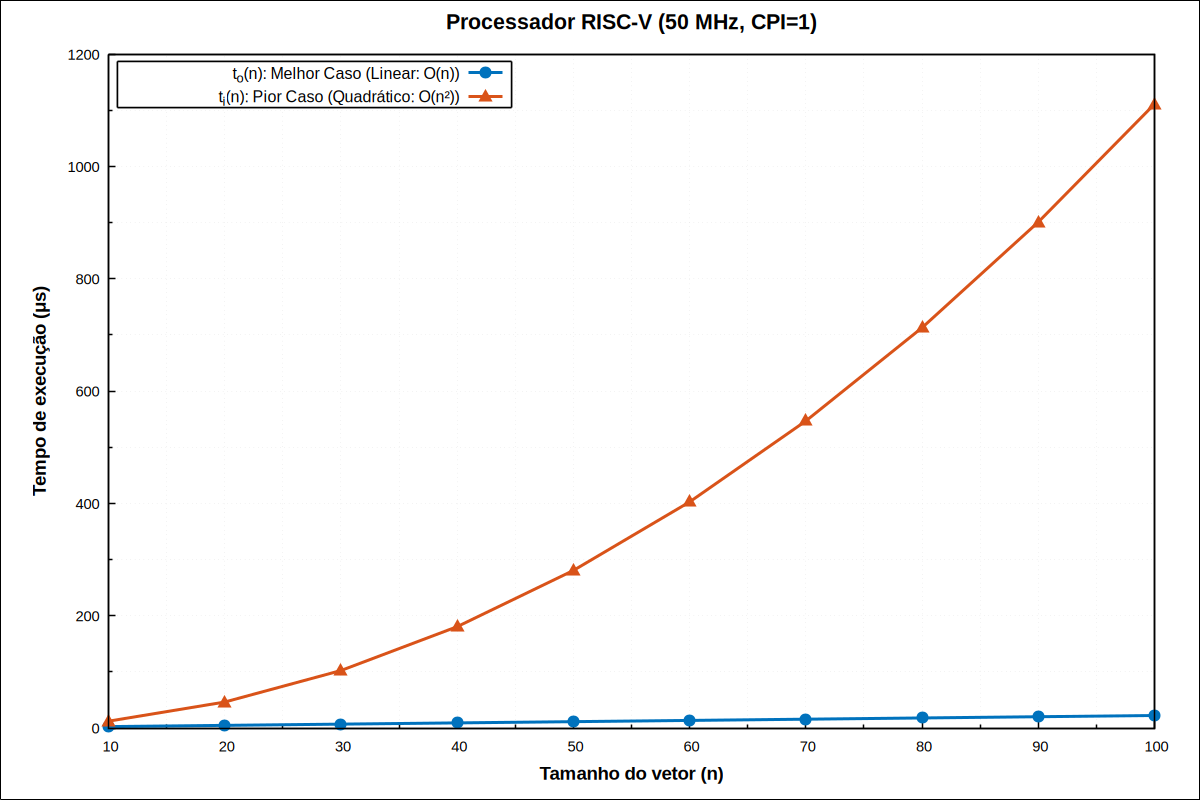
\includegraphics[width=0.8\textwidth]{grafico_tempo_execucao.png}
\caption{Tempo de execução vs. tamanho do vetor n para melhor e pior caso.}
\label{fig:tempo_execucao}
\end{figure}

\subsubsection*{Análise dos Resultados}

Conforme observado na Figura \ref{fig:tempo_execucao}, a curva de melhor caso ($t_o(n)$) demonstra um crescimento linear em relação a $n$, resultado direto da equação $t_o(n) = \frac{11n + 14}{50}$. Em contraste, a curva de pior caso ($t_i(n)$) apresenta um crescimento quadrático, tornando-se significativamente maior à medida que $n$ aumenta, conforme esperado pela equação $t_i(n) = \frac{\frac{11}{2}n^{2} + \frac{11}{2}n + 3}{50}$. 

Esta análise ressalta a sensibilidade do algoritmo de ordenação à disposição inicial dos dados, sendo muito eficiente para entradas quase ordenadas, mas impraticável para entradas grandes e inversamente ordenadas. Por exemplo, para $n=100$, o tempo do pior caso ($1111.06\,\mu s$) é aproximadamente 50 vezes maior que o tempo do melhor caso ($22.28\,\mu s$).

% -----------------------------
% SEÇÃO 2 - COMPILADOR CRUZADO
% -----------------------------
\section*{2) Compilador cruzado GCC}
\addcontentsline{toc}{section}{2) Compilador cruzado GCC}

Um compilador cruzado (\textit{cross compiler}) compila um código fonte para uma arquitetura diferente daquela da máquina em que está sendo utilizado. Você pode baixar gratuitamente os compiladores gcc para todas as arquiteturas (RISC-V, ARM, MIPS, x86 etc.) e instalar na sua máquina, sendo que o código executável gerado apenas poderá ser executado em uma máquina que possuir o processador para qual foi compilado. No gcc, a diretiva de compilação \texttt{-S} faz com que o processo pare com a geração do arquivo em Assembly e a diretiva \texttt{-march} permite definir a arquitetura a ser utilizada.

\textbf{Exemplos:}
\begin{verbatim}
riscv64-unknown-elf-gcc -S -march=rv32imf -mabi=ilp32f  # RV32IMF
arm-eabi-gcc -S -march=armv7                            # ARMv7
gcc -S -m32                                              # x86 32-bit
\end{verbatim}

\subsection*{2.1 Enunciado}

Dado o programa \texttt{sortc.c}, compile-o com a diretiva \texttt{-O0} e obtenha o arquivo \texttt{sortc.s}. Indique as modificações necessárias no código Assembly gerado para que possa ser executado corretamente no Rars. 

\textbf{Dica:} Uso de Assembly em um programa em C. Use a função \texttt{show} definida no \texttt{sort.s} para não precisar implementar a função \texttt{printf}, conforme mostrado no \texttt{sortc\_mod.c}.

\subsection*{2.2 Modificações Necessárias no Código Assembly Gerado (-O0)}
Para executar o código Assembly gerado pelo compilador (com diretiva -O0) no RARS, as seguintes modificações foram necessárias:
\begin{enumerate}
    \item \textbf{Substituição de chamadas de funções:} A instrução \texttt{call} gerada pelo compilador não é suportada diretamente pelo RARS. É necessário substituí-la por \texttt{jal ra, function\_name}.
    \item \textbf{Substituição de argumentos:} O compilador online gerou \texttt{.LANCHOR0} em diversos casos para se referir ao vetor. Não sendo suportado pelo RARS e necessitando da troca pelo vetor \texttt{v} declarado.
    \item \textbf{Ajustes nos endereços de memória:} O código gerado utiliza diretivas como \texttt{\%hi} e \texttt{\%lo} para carregar endereços. No RARS, é mais prático usar a pseudoinstrução \texttt{la} (load address), mas o RARS entende a chamada mesmo assim.
    \item \textbf{Adição de chamada de sistema para encerramento:} No RARS, é necessário adicionar uma chamada de sistema para encerrar o programa corretamente. O compilador não os adiciona.
    \begin{lstlisting}[language=Assembly]
li a7, 10
ecall
    \end{lstlisting}
    \item \textbf{Simplificação do gerenciamento de pilha:} O código gerado pelo compilador com -O0 faz uso excessivo da pilha, o que pode ser simplificado para melhorar o desempenho.
    \item \textbf{Adaptação da função show:} A função \texttt{show} foi adaptada para usar \texttt{ecall} do RARS para a impressão dos valores, ao invés de chamar a função \texttt{printf} do C.
    \item \textbf{Remoção de instruções \texttt{nop} desnecessárias:} O compilador gerou instruções \texttt{nop} para alinhamento, que podem ser removidas no RARS.
\end{enumerate}

\subsection*{2.3 Comparação entre Diferentes Níveis de Otimização}
Foram analisados três arquivos Assembly gerados com diferentes níveis de otimização:

\begin{table}[h!]
    \centering
    \small
    \begin{tabular}{|l|l|r|r|}
        \hline
        \textbf{Arquivo} & \textbf{Otimização} & \textbf{Instruções} & \textbf{Tamanho} \\
        \hline
        2\_3\_O0.asm & -O0 (Sem otimização) & 10103 & 3.817 bytes \\
        2\_3\_O3.asm & -O3 (Otimização máxima) & 2484 & 2.152 bytes \\
        2\_3\_Os.asm & -Os (Otimização p/ tamanho) & 4406 & 2.543 bytes \\
        \hline
    \end{tabular}
    \caption{Comparativo entre diferentes níveis de otimização}
\end{table}

A Figura \ref{fig:otimizacao_comparacao} apresenta uma visualização gráfica dos dados da Tabela 5, permitindo uma comparação imediata do impacto de cada nível de otimização tanto no número de instruções executadas quanto no tamanho do arquivo gerado.

\begin{figure}[H]
\centering
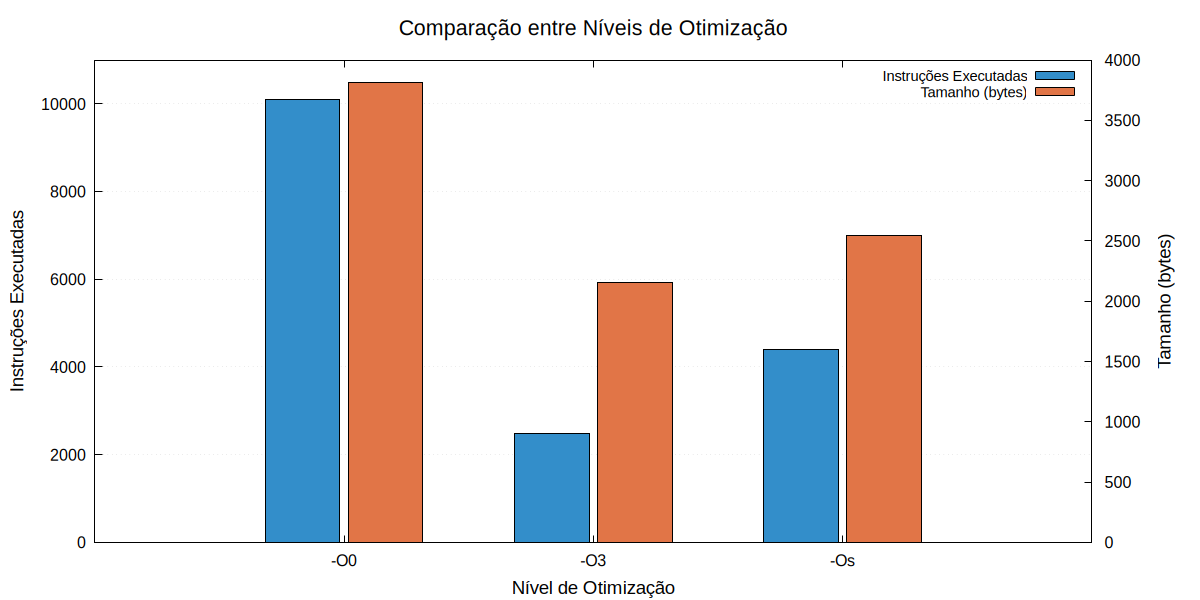
\includegraphics[width=0.85\textwidth]{grafico_otimizacao_comparacao.png}
\caption{Comparação visual entre níveis de otimização: número de instruções e tamanho do arquivo.}
\label{fig:otimizacao_comparacao}
\end{figure}

Observa-se que a otimização \texttt{-O3} apresenta a melhor performance em termos de instruções executadas (redução de 75\%), enquanto \texttt{-Os} oferece o melhor compromisso entre tamanho e desempenho.

\subsection*{2.4 Análise do Código Sem Otimização (-O0)}
\begin{lstlisting}[language=Assembly, caption={Código Assembly gerado com -O0}]
.data
v:
.word 9, 2, 5, 1, 8, 2, 4, 3, 6, 7
.word 10, 2, 32, 54, 2, 12, 6, 3, 1, 78
.word 54, 23, 1, 54, 2, 65, 3, 6, 55, 31

.text
main:
addi sp, sp, -16
sw ra, 12(sp)
sw s0, 8(sp)
addi s0, sp, 16
li a1, 30
lui a5, %hi(v)
addi a0, a5, %lo(v)
call show
li a1, 30
lui a5, %hi(v)
addi a0, a5, %lo(v)
call sort
li a1, 30
lui a5, %hi(v)
addi a0, a5, %lo(v)
call show
li a5, 0
mv a0, a5
lw ra, 12(sp)
lw s0, 8(sp)
addi sp, sp, 16
li a7, 10
ecall

show:
addi sp, sp, -32
sw ra, 28(sp)
sw s0, 24(sp)
addi s0, sp, 32
sw a0, -20(s0)
sw a1, -24(s0)
lw a5, -20(s0)
lw a4, -24(s0)
mv t0, a5
mv t1, a4
mv t2, zero
loop1:
beq t2, t1, fim1
li a7, 1
lw a0, 0(t0)
ecall
li a7, 11
li a0, 9
ecall
addi t0, t0, 4
addi t2, t2, 1
j loop1
fim1:
li a7, 11
li a0, 10
ecall
nop
lw ra, 28(sp)
lw s0, 24(sp)
addi sp, sp, 32
jr ra

swap:
addi sp, sp, -48
sw ra, 44(sp)
sw s0, 40(sp)
addi s0, sp, 48
sw a0, -36(s0)
sw a1, -40(s0)
lw a5, -40(s0)
slli a5, a5, 2
lw a4, -36(s0)
add a5, a4, a5
lw a5, 0(a5)
sw a5, -20(s0)
lw a5, -40(s0)
addi a5, a5, 1
slli a5, a5, 2
lw a4, -36(s0)
add a4, a4, a5
lw a5, -40(s0)
slli a5, a5, 2
lw a3, -36(s0)
add a5, a3, a5
lw a4, 0(a4)
sw a4, 0(a5)
lw a5, -40(s0)
addi a5, a5, 1
slli a5, a5, 2
lw a4, -36(s0)
add a5, a4, a5
lw a4, -20(s0)
sw a4, 0(a5)
nop
lw ra, 44(sp)
lw s0, 40(sp)
addi sp, sp, 48
jr ra

sort:
addi sp, sp, -48
sw ra, 44(sp)
sw s0, 40(sp)
addi s0, sp, 48
sw a0, -36(s0)
sw a1, -40(s0)
sw zero, -20(s0)
j .L4
.L8:
lw a5, -20(s0)
addi a5, a5, -1
sw a5, -24(s0)
j .L5
.L7:
lw a1, -24(s0)
lw a0, -36(s0)
call swap
lw a5, -24(s0)
addi a5, a5, -1
sw a5, -24(s0)
.L5:
lw a5, -24(s0)
blt a5, zero, .L6
lw a5, -24(s0)
slli a5, a5, 2
lw a4, -36(s0)
add a5, a4, a5
lw a4, 0(a5)
lw a5, -24(s0)
addi a5, a5, 1
slli a5, a5, 2
lw a3, -36(s0)
add a5, a3, a5
lw a5, 0(a5)
bgt a4, a5, .L7
.L6:
lw a5, -20(s0)
addi a5, a5, 1
sw a5, -20(s0)
.L4:
lw a4, -20(s0)
lw a5, -40(s0)
blt a4, a5, .L8
nop
nop
lw ra, 44(sp)
lw s0, 40(sp)
addi sp, sp, 48
jr ra
\end{lstlisting}

\subsection*{2.5 Análise do Código com Otimização Máxima (-O3)}
\begin{lstlisting}[language=Assembly, caption={Código Assembly gerado com -O3}]
.data
v:
.word 9, 2, 5, 1, 8, 2, 4, 3, 6, 7
.word 10, 2, 32, 54, 2, 12, 6, 3, 1, 78
.word 54, 23, 1, 54, 2, 65, 3, 6, 55, 31

.text
main:
# Carrega o endereco do vetor v
la a0, v
li a1, 30
# Primeira chamada da funcao show
jal ra, show
# Chama a funcao sort
la a0, v
li a1, 30
jal ra, sort
# Segunda chamada da funcao show
la a0, v
li a1, 30
jal ra, show
# Retorno da funcao main
li a0, 0
ret

show:
mv t0, a0
mv t1, a1
mv t2, zero
show_loop:
beq t2, t1, show_fim
li a7, 1
lw a0, 0(t0)
ecall
li a7, 11
li a0, 9
ecall
addi t0, t0, 4
addi t2, t2, 1
j show_loop
show_fim:
li a7, 11
li a0, 10
ecall
ret

swap:
slli a1, a1, 2
add a0, a0, a1
lw a4, 0(a0)
lw a5, 4(a0)
sw a5, 0(a0)
sw a4, 4(a0)
ret

sort:
ble a1, zero, .L4
li a6, -1
add a7, a1, a6
mv a1, a6
.L7:
mv a4, a6
mv a5, a0
bne a6, a1, .L6
j .L8
.L9:
lw t0, -4(a5)
lw t1, 0(a5)
sw t1, -4(a5)
sw t0, 0(a5)
addi a5, a5, -4
beq a4, a1, .L8
.L6:
lw a2, -4(a5)
lw a3, 0(a5)
addi a4, a4, -1
bgt a2, a3, .L9
.L8:
addi a6, a6, 1
addi a0, a0, 4
bne a7, a6, .L7
ret
.L4:
ret
\end{lstlisting}

\subsection*{2.6 Análise do Código com Otimização para Tamanho (-Os)}
\begin{lstlisting}[language=Assembly, caption={Código Assembly gerado com -Os}]
.data
v:
.word 9, 2, 5, 1, 8, 2, 4, 3, 6, 7
.word 10, 2, 32, 54, 2, 12, 6, 3, 1, 78
.word 54, 23, 1, 54, 2, 65, 3, 6, 55, 31

.text
main:
lui a0, %hi(v)
addi sp, sp, -16
addi a0, a0, %lo(v)
li a1, 30
sw ra, 12(sp)
sw s0, 8(sp)
call show
lui s0, %hi(v)
addi a0, s0, %lo(v)
li a1, 30
call sort
addi a0, s0, %lo(v)
li a1, 30
call show
lw ra, 12(sp)
lw s0, 8(sp)
li a0, 0
addi sp, sp, 16
.set .LANCHOR0, v
li a7, 10
ecall

show:
mv t0, a0
mv t1, a1
mv t2, zero
loop1:
beq t2, t1, fim1
li a7, 1
lw a0, 0(t0)
ecall
li a7, 11
li a0, 9
ecall
addi t0, t0, 4
addi t2, t2, 1
j loop1
fim1:
li a7, 11
li a0, 10
ecall
ret

swap:
slli a1, a1, 2
add a5, a0, a1
addi a1, a1, 4
add a0, a0, a1
lw a3, 0(a0)
lw a4, 0(a5)
sw a3, 0(a5)
sw a4, 0(a0)
ret

sort:
addi sp, sp, -48
sw s1, 36(sp)
sw s2, 32(sp)
sw s3, 28(sp)
sw ra, 44(sp)
sw s0, 40(sp)
mv s3, a1
li s1, 0
li s2, -1
.L4:
blt s1, s3, .L9
lw ra, 44(sp)
lw s0, 40(sp)
lw s1, 36(sp)
lw s2, 32(sp)
lw s3, 28(sp)
addi sp, sp, 48
jr ra
.L9:
slli s0, s1, 2
addi a1, s1, -1
add s0, a0, s0
.L5:
bne a1, s2, .L6
.L8:
addi s1, s1, 1
j .L4
.L6:
lw a4, -4(s0)
addi s0, s0, -4
lw a5, 4(s0)
ble a4, a5, .L8
sw a1, 12(sp)
sw a0, 8(sp)
call swap
lw a1, 12(sp)
lw a0, 8(sp)
addi a1, a1, -1
j .L5
\end{lstlisting}

\subsection*{2.7 Conclusões}
\begin{enumerate}
    \item \textbf{Impacto da Otimização:} A otimização -O3 reduziu o número de instruções executadas em aproximadamente 75\% em relação ao código sem otimização (-O0), demonstrando a eficácia das técnicas de otimização do compilador.
    \item \textbf{Compromisso Tamanho vs. Desempenho:} A otimização -Os oferece um equilíbrio interessante, tendo um número de instruções aproximadamente 32\% menor que o código não otimizado, mas ainda 77\% maior que o código com otimização máxima.
    \item \textbf{Adaptação para RARS:} O código gerado pelo compilador precisa ser adaptado para funcionar corretamente no simulador RARS. Isso inclui modificações nas chamadas de função, acesso à memória e uso das chamadas de sistema do RARS.
    \item \textbf{Benefícios Educacionais:} A comparação entre os diferentes níveis de otimização fornece insights valiosos sobre as estratégias empregadas pelos compiladores modernos para melhorar o desempenho do código. As modificações necessárias para executar o código no RARS demonstram as diferenças entre o assembly gerado para um sistema real e o ambiente de simulação, destacando a importância de compreender as convenções de chamada de função e o modelo de execução de um processador RISC-V.
\end{enumerate}

\subsection*{2.8 Relatório Comparativo - Código RISC-V -O0 vs -O1}
\subsubsection*{Introdução}
Este relatório apresenta uma análise comparativa entre código RISC-V compilado com diferentes níveis de otimização: -O0 (sem otimização) e -O1 (otimização básica). O objetivo é demonstrar o impacto das otimizações de compilador no número de instruções e ciclos de execução.

\subsection*{Código sem Otimização (-O0)}
Com o nível de otimização -O0, o compilador gera código sem qualquer otimização, mantendo funções separadas com chamadas explícitas:
\begin{lstlisting}[language=Assembly]
.data
newline: .asciz "\n"
space: .asciz " "
.text
.globl main
main:
li a0, 7
mv a1, a0
...
# funcoes f1_label a f6_label abaixo
f1_label:
slli a0, a0, 2
ret
f2_label:
slli a0, a0, 2
ret
f3_label:
add a0, a0, a0
add a0, a0, a0
ret
f4_label:
li t0, 3
mul t1, a0, t0
add a0, t1, a0
ret
f5_label:
slli t0, a0, 1
slli t1, a0, 1
add a0, t0, t1
ret
f6_label:
li t0, 4
mul a0, a0, t0
ret
\end{lstlisting}

\subsection*{Saída do Terminal (-O0)}
Ao executar o código sem otimização, obtemos os seguintes resultados para número de instruções e ciclos:
\begin{verbatim}
5 5
5 5
6 6
7 7
7 7
6 6
\end{verbatim}

\subsection*{Código com Otimização (-O1)}
Com o nível de otimização -O1, o compilador aplica otimizações básicas, incluindo inline de funções:
\begin{lstlisting}[language=Assembly]
.data
newline: .asciz "\n"
space: .asciz " "
.text
.globl main
main:
li a0, 7
...
# funcoes inline para f1 a f6
f1: slli a0, a0, 2
f2: slli a0, a0, 2
f3: add a0, a0, a0 ; add a0, a0, a0
f4: li t0, 3 ; mul t1, a0, t0 ; add a0, t1, a0
f5: slli t0, a0, 1 ; slli t1, a0, 1 ; add a0, t0, t1
f6: li t0, 4 ; mul a0, a0, t0
\end{lstlisting}

\subsection*{5.1 Saída do Terminal (-O1)}
Ao executar o código com otimização básica, obtemos os seguintes resultados:
\begin{verbatim}
3 3
3 3
4 4
5 5
5 5
4 4
\end{verbatim}

\subsection*{Análise Comparativa}
\subsubsection*{Observações sobre a Medição}
Os números exibidos no terminal do RARS refletem o custo total da execução da função, incluindo as instruções de medição (\texttt{csrr}), chamada com \texttt{jal}, a execução da função em si, e o \texttt{ret}. Ou seja, o valor inclui mais do que apenas o conteúdo da função.
Apesar disso, essa medição é válida para comparar o desempenho relativo entre as implementações, especialmente quando usamos o mesmo padrão de medição para todas.

\subsubsection*{2.8.2 Tabela de Resultados}
\begin{table}[h!]
    \centering
    \begin{tabular}{|l|l|l|c|c|}
        \hline
        \textbf{Função} & \textbf{Otimização} & \textbf{Implementação} & \textbf{Instruções} & \textbf{Ciclos} \\
        \hline
        f1 & -O0 & Função separada & 5 & 5 \\
        f1 & -O1 & Inline & 3 & 3 \\
        \hline
        f2 & -O0 & Função separada & 5 & 5 \\
        f2 & -O1 & Inline & 3 & 3 \\
        \hline
        f3 & -O0 & Função separada & 6 & 6 \\
        f3 & -O1 & Inline & 4 & 4 \\
        \hline
        f4 & -O0 & Função separada & 7 & 7 \\
        f4 & -O1 & Inline & 5 & 5 \\
        \hline
        f5 & -O0 & Função separada & 7 & 7 \\
        f5 & -O1 & Inline & 5 & 5 \\
        \hline
        f6 & -O0 & Função separada & 6 & 6 \\
        f6 & -O1 & Inline & 4 & 4 \\
        \hline
    \end{tabular}
    \caption{Comparação de instruções e ciclos entre implementações com e sem otimização}
\end{table}

A Figura \ref{fig:otimizacao_funcoes} ilustra graficamente a comparação entre as versões \texttt{-O0} e \texttt{-O1}, tornando evidente a redução consistente no número de instruções para todas as funções analisadas.

\begin{figure}[H]
\centering
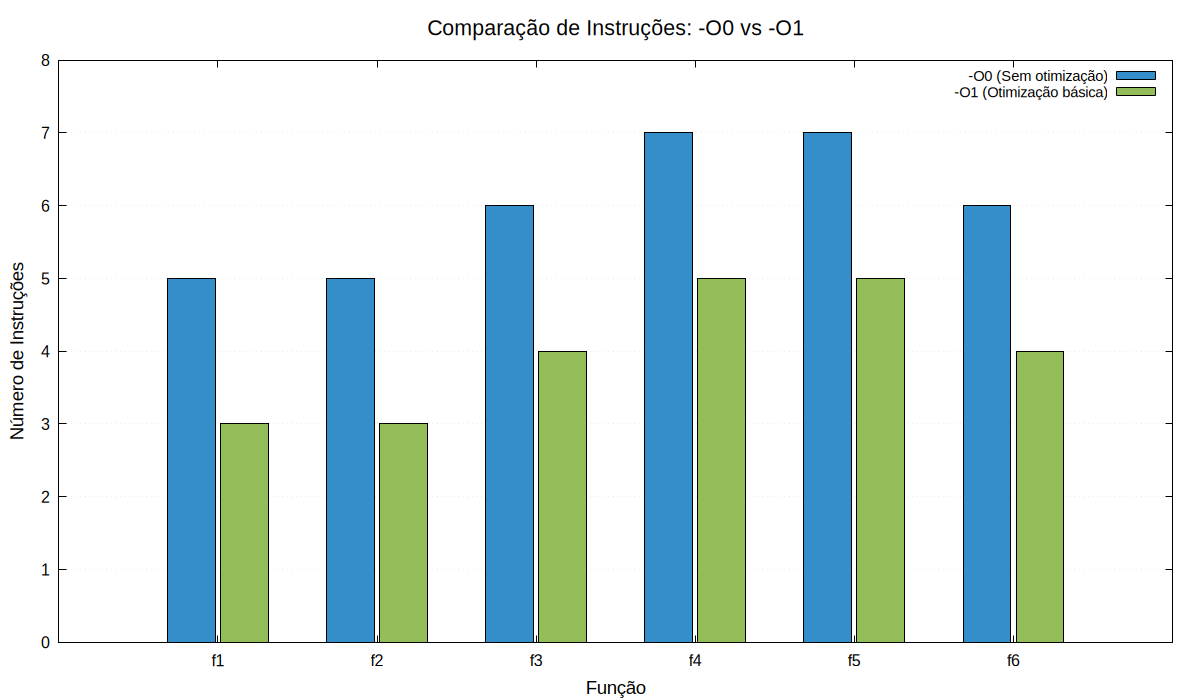
\includegraphics[width=0.85\textwidth]{grafico_otimizacao_funcoes.png}
\caption{Comparação visual do número de instruções por função nos níveis -O0 e -O1.}
\label{fig:otimizacao_funcoes}
\end{figure}

\subsubsection*{2.8.3 Análise Visual}

Como pode ser observado na Figura \ref{fig:otimizacao_funcoes}, todas as funções apresentam uma redução uniforme de 2 instruções ao passar de \texttt{-O0} para \texttt{-O1}. Esta redução é resultado direto da eliminação das instruções de controle de fluxo (\texttt{jal} e \texttt{ret}) através do inlining de funções.

\subsubsection*{2.8.4 Gráfico Comparativo (Análise Textual)}
\paragraph{Detalhamento das Otimizações}
\paragraph{Eliminação de Instruções de Controle}
A principal otimização observada na passagem de -O0 para -O1 é a eliminação das instruções de controle de fluxo:
\begin{itemize}
    \item Sem o \texttt{jal}: Economiza uma instrução de chamada de função
    \item Sem o \texttt{ret}: Economiza uma instrução de retorno de função
\end{itemize}
Isto explica a redução de 2 instruções em todas as funções analisadas.

\paragraph{Representação Numérica da Redução}
Além do inlining, outras otimizações poderiam ser aplicadas em níveis mais altos:
\begin{itemize}
    \item Substituição de operações de multiplicação por deslocamentos quando o multiplicador é uma potência de 2
    \item Combinação de múltiplas instruções em uma única instrução mais eficiente
    \item Eliminação de registradores temporários desnecessários
\end{itemize}

\subsubsection*{2.8.5 Conclusão}
A comparação entre as versões -O0 e -O1 (simulada com código inline) demonstra que as otimizações de compilação reduzem significativamente o número de instruções e ciclos. Isso acontece principalmente pela eliminação da sobrecarga das chamadas de função (jal/ret) e pela substituição de múltiplas instruções por instruções mais diretas e eficientes, como \texttt{slli}.
A média de economia é de aproximadamente 2 instruções por função analisada, o que representa uma redução de:
\begin{itemize}
    \item 40\% para as funções f1 e f2
    \item 33\% para as funções f3 e f6
    \item 29\% para as funções f4 e f5
\end{itemize}
Esta análise demonstra que mesmo o nível básico de otimização (-O1) já proporciona ganhos significativos de performance, especialmente para funções pequenas onde o custo relativo das chamadas de função é maior.

\subsection*{2.9 Níveis de Otimização em Compiladores GCC/Clang}
\subsubsection*{Introdução}
Os compiladores modernos como GCC e Clang oferecem diferentes níveis de otimização que podem ser aplicados ao código-fonte durante a compilação. Esses níveis são controlados por flags como \texttt{-O0}, \texttt{-O1}, \texttt{-O2}, \texttt{-O3} e \texttt{-Os}. Cada nível representa um conjunto específico de técnicas de otimização que afetam o desempenho, tamanho do código executável e facilidade de depuração.

\subsubsection*{2.9.1 Descrição dos Níveis de Otimização}

\paragraph{-O0 (Sem Otimização)}
\textbf{Descrição:} Desativa completamente todas as otimizações.
\textbf{Características:}
\begin{itemize}
    \item Compilação muito rápida
    \item Código gerado é diretamente mapeável ao código fonte
    \item Todas as variáveis são armazenadas na memória (não em registradores)
    \item Operações são executadas na ordem exata especificada no código
\end{itemize}
\textbf{Uso recomendado:} Durante desenvolvimento e depuração, quando é importante que o comportamento do programa corresponda exatamente ao código fonte.

\subsubsection*{-O1 (Otimização Básica)}
\textbf{Descrição:} Aplica otimizações básicas que não demandam muito tempo de compilação.
\textbf{Características:}
\begin{itemize}
    \item Eliminação de código morto
    \item Eliminação de expressões redundantes
    \item Otimizações simples de fluxo de controle
    \item Melhora significativa de performance em relação a -O0
    \item Ainda mantém boa correspondência com o código-fonte para depuração
\end{itemize}
\textbf{Uso recomendado:} Para desenvolvimento quando se deseja um equilíbrio entre tempo de compilação, facilidade de depuração e performance.

\paragraph{-O2 (Otimização Moderada)}
\textbf{Descrição:} Inclui todas as otimizações de -O1 mais otimizações adicionais sem comprometer significativamente o tempo de compilação.
\textbf{Características:}
\begin{itemize}
    \item Alinhamento de funções, loops e saltos
    \item Otimizações mais agressivas de instrução e cache
    \item Não realiza trocas entre tamanho e velocidade
    \item Significativamente mais rápido que -O1 na execução
    \item Equilibra tempo de compilação e performance
\end{itemize}
\textbf{Uso recomendado:} Para builds de produção na maioria dos casos; considerado o nível padrão para distribuição de software.

\paragraph{-O3 (Otimização Agressiva)}
\textbf{Descrição:} Inclui todas as otimizações de -O2 e adiciona otimizações mais agressivas.
\textbf{Características:}
\begin{itemize}
    \item Inlining agressivo de funções
    \item Desenrolamento de loops (loop unrolling)
    \item Vetorização automática
    \item Otimizações matemáticas avançadas
    \item Pode aumentar significativamente o tamanho do executável
    \item Compilação mais lenta
    \item Nem sempre resulta em código mais rápido (pode degradar a performance devido ao uso ineficiente de cache)
\end{itemize}
\textbf{Uso recomendado:} Para código com cálculos matemáticos intensivos, processamento de sinais e aplicações onde o desempenho máximo é crítico.

\paragraph{-Os (Otimização para Tamanho)}
\textbf{Descrição:} Similar a -O2, mas prioriza a redução do tamanho do executável.
\textbf{Características:}
\begin{itemize}
    \item Desativa otimizações que aumentam significativamente o tamanho do código
    \item Realiza otimizações específicas para reduzir o tamanho do executável
    \item Geralmente produz código menor que -O1, -O2 e -O3
    \item Performance geralmente entre -O1 e -O2
\end{itemize}
\textbf{Uso recomendado:} Para sistemas embarcados, dispositivos com memória limitada ou quando o tamanho do executável é crítico.

\subsubsection*{2.9.2 Comparação dos Níveis de Otimização}
\begin{table}[h!]
    \centering
    \small
    \begin{tabular}{|c|c|c|c|c|}
        \hline
        \textbf{Nível} & \textbf{Tempo de} & \textbf{Tamanho do} & \textbf{Performance} & \textbf{Facilidade de} \\
        & \textbf{Compilação} & \textbf{Executável} & & \textbf{Depuração} \\
        \hline
        -O0 & Muito Rápido & Grande & Baixa & Excelente \\
        -O1 & Rápido & Médio & Média & Boa \\
        -O2 & Moderado & Médio & Alta & Moderada \\
        -O3 & Lento & Grande & Muito Alta* & Difícil \\
        -Os & Moderado & Pequeno & Média-Alta & Moderada \\
        \hline
    \end{tabular}
    \caption{Comparação dos níveis de otimização}
\end{table}

\noindent\textit{* O nível -O3 nem sempre resulta em melhor performance do que -O2 em todos os casos.}

\subsection*{2.10 Técnicas de Otimização Aplicadas em Cada Nível}
Aqui estão algumas das técnicas específicas aplicadas em cada nível de otimização:
\begin{itemize}[leftmargin=*]
    \item \textbf{-O1 inclui:}
    \begin{itemize}
        \item Propagação constante (constant propagation)
        \item Eliminação de código morto (dead code elimination)
        \item Eliminação de subexpressões comuns (common subexpression elimination)
        \item Otimização de instruções de salto (jump optimization)
    \end{itemize}
    \item \textbf{-O2 adiciona:}
    \begin{itemize}
        \item Otimização de alinhamento de memória
        \item Análise de alcance de variáveis
        \item Reordenação de instruções
        \item Otimização de ramificação condicional
        \item Eliminação de variáveis não utilizadas
        \item Propagação de cópias (copy propagation)
    \end{itemize}
    \item \textbf{-O3 adiciona:}
    \begin{itemize}
        \item Inline de funções mais agressivo
        \item Desenrolamento de loops (loop unrolling)
        \item Auto-vetorização (transformação de código escalar em código vetorial)
        \item Pré-computação de expressões
        \item Otimização de ramificação preditiva
    \end{itemize}
    \item \textbf{-Os é similar a -O2, mas:}
    \begin{itemize}
        \item Desativa otimizações que aumentam tamanho significativamente
        \item Prioriza instruções mais compactas
        \item Reduz tamanho de alinhamentos de memória
        \item Evita desenrolamento de loops e inline excessivo
    \end{itemize}
\end{itemize}

\subsection*{2.11 Exemplos de Uso}
Para compilar um programa C usando diferentes níveis de otimização:
\begin{lstlisting}[language=bash]
# Compilacao sem otimizacao (para depuracao)
gcc -O0 -g programa.c -o programa_debug

# Compilacao com otimizacao moderada (para producao)
gcc -O2 programa.c -o programa_release

# Compilacao com otimizacao agressiva
gcc -O3 programa.c -o programa_performance

# Compilacao com otimizacao para tamanho
gcc -Os programa.c -o programa_pequeno
\end{lstlisting}

\subsection*{2.12 Conclusão}
A escolha do nível de otimização adequado depende do contexto e das necessidades específicas:
\begin{itemize}[leftmargin=*]
    \item Para desenvolvimento e depuração: \texttt{-O0} ou \texttt{-O1}
    \item Para distribuição de software geral: \texttt{-O2}
    \item Para aplicações com cálculos intensivos: \texttt{-O3}
    \item Para sistemas com restrições de memória: \texttt{-Os}
\end{itemize}
É recomendável testar diferentes níveis de otimização para cada aplicação específica, já que o impacto pode variar significativamente dependendo da natureza do código e da arquitetura alvo. Na maioria dos casos, \texttt{-O2} oferece o melhor equilíbrio entre performance e estabilidade para aplicações de uso geral.

% --- fim da seção 2 ---

% -----------------------------
% SEÇÃO 3 - DFT
% -----------------------------
\newpage
\section*{(5.0) 3) Transformada Discreta de Fourier (DFT)}
\addcontentsline{toc}{section}{3) Transformada Discreta de Fourier (DFT)}

A Transformada Discreta de Fourier (DFT) converte os sinais amostrados no domínio do tempo (amostra) para o domínio frequência complexa (espectro) e é definida por
\[
X[k] = \sum_{n=0}^{N-1} x[n] e^{-2\pi i \frac{k n}{N}}
\]
onde $x[n]$ são as amostras do sinal x no domínio do tempo, $X[k]$ são as amostras complexas do espectro no domínio frequência, $N$ é o número de pontos e $i=\sqrt{-1}$. \\
Dica: fórmula de Euler $e^{i\theta} = \cos(\theta) + i\sin(\theta)$.

\subsection*{(0.5) 3.1) Escreva um procedimento que receba um ângulo em radianos (em \texttt{fa0}) e retorne $\cos(\theta)$ (em \texttt{fa0}) e $\sin(\theta)$ (em \texttt{fa1}).}
\addcontentsline{toc}{subsection}{3.1) SINCOS}

\{\texttt{fa0,fa1}\} = \texttt{sincos(float theta)}. \\
Dica: use aproximação por séries para o cálculo das funções trigonométricas.

\section*{Resposta à Questão 3.1}
\addcontentsline{toc}{section}{Resposta à Questão 3.1}

\subsection*{Método}
Implementamos um procedimento \texttt{SINCOS} em Assembly RISC-V (RV32IMF) que calcula $\sin(\theta)$ e $\cos(\theta)$ por aproximação via séries de Taylor, utilizando ponto flutuante em dupla precisão:
\[
\sin(x) = \sum_{n=0}^{\infty} (-1)^n \frac{x^{2n+1}}{(2n+1)!},\qquad
\cos(x) = \sum_{n=0}^{\infty} (-1)^n \frac{x^{2n}}{(2n)!}
\]
Para cada função, somamos um número finito de termos: 10 termos para o seno (termo inicial $\theta$ somado a 10 termos subsequentes de potências ímpares) e 10 termos para o cosseno (termo inicial 1 somado a 10 termos subsequentes de potências pares). Os termos \(x^k/k!\) são formados multiplicando por \(x\) repetidamente (\texttt{POWPREP}) e dividindo pelo fatorial (\texttt{FATPREP}). O sinal alternado é controlado por um acumulador de sinal.

\subsection*{Código}
O código-fonte utilizado encontra-se em \texttt{Arquivos/3.1.asm} e é incluído abaixo para referência.

\begin{lstlisting}[language=Assembly, caption={Procedimento SINCOS em RISC-V: séries de Taylor para seno e cosseno}]
.text

SINCOS:
	addi sp, sp, -80
	fsd fs0, 72(sp)
	fsd fs1, 64(sp)
	fsd fs2, 56(sp)
	fsd fs3, 48(sp)
	fsd fs4, 40(sp)
	sw s0, 36(sp)
	sw s1, 32(sp)
	sw s2, 28(sp)
	sw s3, 24(sp)
	sw s4, 20(sp)
	sw s5, 16(sp)
	sw s6, 12(sp)
	sw s7, 8(sp)
	sw s8, 4(sp)
	sw s9, 0(sp)
	
	mv s10, ra
	fmv.d fs0, fa0
	fcvt.d.w ft4, zero
	li t6, -1
	fcvt.d.w ft6, t6
	li t1, 3
	li s1, 10
	fcvt.d.w ft5, t6
	fcvt.d.w ft1, t1
	fmv.d fs1, fs0
	jal SINPREP
	li s1, 10
	li t1, 1
	fcvt.d.w ft5, t6
	fcvt.d.w fs1, t1
	li t1, 2
	jal COSPREP
	j END

SINPREP:
	mv s2, ra
SIN:
	addi s1, s1, -1
	jal FUNCI
	jal SUM
	addi t1, t1, 2
	bgt s1, zero, SIN
	li t0, -1
	fcvt.d.w ft1, t0
	fmul.d fs1, fs1, ft1
	fmv.d fa1, fs1
	mv ra, s2
	ret

COSPREP:
	mv s2, ra
COS:
	addi s1, s1, -1
	jal FUNCI
	jal SUM
	addi t1, t1, 2
	bgt s1, zero, COS
	fmv.d fa0, fs1
	mv ra, s2
	ret
	
FUNCI:
	mv s3, ra
	mv t2, t1
	li s0, 1
	fmv.d fs2, fs0
	jal FATPREP
	mv t2, t1
	addi t2, t2, -1
	beq t2, zero, CONTINUE
	jal POWPREP
	
CONTINUE:
	fcvt.d.w fs3, s0
	fdiv.d fs2, fs2, fs3
	mv ra, s3
	ret

FATPREP:
	mv s4, ra
FAT:
	fcvt.d.w ft2, t2
	fdiv.d fs2, fs2, ft2
	addi t2, t2, -1
	bgt t2, zero, FAT
	mv ra, s4
	ret
	
POWPREP:
	mv s5, ra
POW:
	fmul.d fs2, fs2, fs0
	addi t2, t2, -1
	bgt t2, zero, POW
	mv ra, s5
	ret
	
SUM:
	fmul.d fs2, fs2, ft5
	fadd.d fs1, fs1, fs2
	fmul.d ft5, ft5, ft6
	ret
	
END:
	lw s9, 0(sp)
    lw s8, 4(sp)
	lw s7, 8(sp)
	lw s6, 12(sp)
	lw s5, 16(sp)
	lw s4, 20(sp)
	lw s3, 24(sp)
	lw s2, 28(sp)
 	lw s1, 32(sp)
	lw s0, 36(sp)
	fld fs4, 40(sp)
	fld fs3, 48(sp)
	fld fs2, 56(sp)
	fld fs1, 64(sp)
	fld fs0, 72(sp)
	addi sp, sp, 80
	
	mv ra, s10
	ret
\end{lstlisting}

\subsection*{Descrição do funcionamento}
\begin{itemize}
    \item \textbf{Entrada:} \texttt{fa0} contém o ângulo em radianos (\(\theta\)).
    \item \textbf{Pré-processamento (label \texttt{SINCOS}):}
    \begin{itemize}
        \item Alocamos todos os registrados usados pelo programa anterior na \textit{stack pointer}.
        \item Copiamos \(\theta\) para \texttt{fs0} (\textit{argumento base}).
        \item Definimos variáveis de controle: \texttt{t1} armazena o expoente atual (começa em 3 para seno e em 2 para cosseno), \texttt{s1} é o contador de termos a somar, \texttt{ft5} guarda o sinal acumulado (\(+1\) ou \(-1\)) e \texttt{ft6} vale \(-1\) para alternância de sinal.
    \end{itemize}
    \item \textbf{Laços de soma} (\texttt{SINPREP}/\texttt{COSPREP}): em cada iteração, chamamos \texttt{FUNCI} para construir o termo \(x^{t1}/t1!\) em \texttt{fs2}, então \texttt{SUM} acumula em \texttt{fs1} com o sinal correto e alterna o sinal para a próxima iteração. O expoente \texttt{t1} é incrementado de 2 em 2, gerando apenas potências ímpares (seno) ou pares (cosseno) conforme a preparação.
    \item \textbf{Cálculo do termo} (\texttt{SINI}):
    \begin{itemize}
        \item Inicializa \texttt{fs2} com \(x\) (\texttt{fs0}).
        \item \texttt{FATPREP} divide sucessivamente por \(t1, t1-1, \dots, 1\) para produzir \(x/t1!\).
        \item Se \(t1>1\), \texttt{POWPREP} multiplica por \(x\) \(t1-1\) vezes para obter \(x^{t1}/t1!\).
    \end{itemize}
    \item \textbf{Acúmulo e alternância} (\texttt{SUM}): \texttt{fs2} é multiplicado por \texttt{ft5} (sinal), somado ao acumulador \texttt{fs1}, e então \texttt{ft5} é multiplicado por \texttt{ft6} para alternar o sinal.
    \item \textbf{Saída:} ao final, o código move os resultados para registradores de retorno: \texttt{fa0} recebe o valor acumulado do cosseno e \texttt{fa1} o do seno. Em seguida, realocamos todos os registrados do progama anterior novamente para retornarmos.
\end{itemize}

\paragraph{Mapeamento de registradores principais}
\begin{itemize}
    \item \texttt{fs0}: \(x=\theta\) (entrada)
    \item \texttt{fs1}: acumulador da série (resultado parcial/final)
    \item \texttt{fs2}: termo corrente \(x^{k}/k!\)
    \item \texttt{ft5}: sinal acumulado (inicia em $+1$ para seno e $-1$ para cosseno)
    \item \texttt{ft6}: constante $-1$ para alternância de sinal
    \item \texttt{t1}: expoente atual (\(k\)), cresce de 2 em 2
    \item \texttt{s1}: contador de termos a somar em cada série
\end{itemize}

\subsection*{(1.0) 3.2) Escreva um procedimento em Assembly RISC-V com a seguinte definição:}
\addcontentsline{toc}{subsection}{3.2) DFT}

\begin{verbatim}
void DFT(float *x, float *X_real, float *X_imag, int N)
\end{verbatim}
que dado o endereço do vetor $x[n]$ de floats (em \texttt{a0}) de tamanho $N$ na memória, os endereços dos espaços reservados para o vetor complexo $X[k]$ (parte real e parte imaginária) (em \texttt{a1} e \texttt{a2}) e o número de pontos $N$ (em \texttt{a3}), calcule a DFT de $N$ pontos de $x[n]$ e coloque o resultado no espaço alocado para \texttt{X\_real[k]} e \texttt{X\_imag[k]}.

\section*{Resposta à Questão 3.2}
\addcontentsline{toc}{section}{Resposta à Questão 3.2}

\subsection*{Método}
Implementamos o procedimento \texttt{DFT(float *x, float *X\_real, float *X\_imag, int N)} em Assembly RISC-V (RV32IMF) conforme o arquivo oficial \texttt{Arquivos/Q3/3.2/3.2.asm}. Esta versão opera em \textbf{dupla precisão} (registradores \texttt{fd*}, instruções \texttt{.d}) e utiliza a seguinte abordagem:

\paragraph{Interface e estrutura:}
\begin{itemize}
  \item \textbf{Entradas:} \texttt{a0} = endereço de \texttt{x[]} (array de doubles), \texttt{a1} = endereço de \texttt{X\_real[]}, \texttt{a2} = endereço de \texttt{X\_imag[]}, \texttt{a3} = \texttt{N} (número de pontos).
  \item \textbf{Constante angular:} \texttt{PIK = -0.785398163397448309} ($\approx -\pi/4$), adequada para $N=8$ (caso típico do enunciado). O sinal negativo reflete a exponencial complexa $e^{-j\theta}$ da DFT.
  \item \textbf{Cálculo de $\theta$:} O label \texttt{THETA} computa $\theta = ((k \cdot n) \bmod N) \times \texttt{PIK}$ e retorna o ângulo em \texttt{fa0}. Isso evita calcular $2\pi k n / N$ diretamente, aproveitando a periodicidade e a constante pré-calculada.
  \item \textbf{Estrutura de laços aninhados:}
    \begin{itemize}
      \item \textbf{Laço externo} (\texttt{PREPFORK}/\texttt{FORK}): itera sobre $k = 0 \dots N-1$ (índice de frequência).
      \item \textbf{Laço interno} (\texttt{PREPSUM}/\texttt{SUMDFT}): itera sobre $n = 0 \dots N-1$ (índice de tempo), acumulando:
      \begin{align*}
        \text{Re}\{X[k]\} &= \sum_{n} x[n] \cos\theta \\
        \text{Im}\{X[k]\} &= \sum_{n} x[n] (-\sin\theta)
      \end{align*}
      Para cada $(k,n)$, chama \texttt{THETA} para obter o ângulo e depois \texttt{SINCOS} (da questão 3.1) para obter $\cos\theta$ (em \texttt{fa0}) e $\sin\theta$ (em \texttt{fa1}).
    \end{itemize}
  \item \textbf{Armazenamento:} O label \texttt{ALLOC} grava as partes real (\texttt{fs3}) e imaginária (\texttt{fs4}) de $X[k]$ nos arrays de saída usando \texttt{fsd} (store double).
  \item \textbf{Dependência:} O código inclui \texttt{3.1.asm} no final, trazendo o procedimento \texttt{SINCOS}.
\end{itemize}

\paragraph{Mapeamento de registradores principais:}
\begin{itemize}
  \item \texttt{s2}: ponteiro para \texttt{x[]}
  \item \texttt{s3}: ponteiro para \texttt{X\_real[]}
  \item \texttt{s4}: ponteiro para \texttt{X\_imag[]}
  \item \texttt{s7}: $N$
  \item \texttt{s0}: índice $k$ (frequência)
  \item \texttt{s1}: índice $n$ (tempo)
  \item \texttt{fs3}: acumulador de parte real
  \item \texttt{fs4}: acumulador de parte imaginária
  \item \texttt{fs1}: valor de $x[n]$ corrente
\end{itemize}

\subsection*{Código (3.2.asm)}
\begin{lstlisting}[language=Assembly, caption={DFT (3.2.asm) — versão oficial em dupla precisão}]
.data
PIK: .double -0.785398163397448309

.text

DFT: 	
	mv s8, ra
	mv s2, a0
	mv s3, a1
	mv s4, a2
	mv s7, a3
	mv s0, zero
	fcvt.d.w fs0, s7
	jal PREPFORK
	mv ra, s8
	ret
	

THETA:
	la t0, PIK
	fld ft0, 0(t0)
	mul t0, s0, s1
	rem t0, t0, s7
	fcvt.d.w ft1, t0
	fmul.d ft1, ft1, ft0
	fmv.d fa0, ft1
	ret
	
PREPFORK:
	mv s6, ra
FORK:	
	fcvt.d.w fs3, zero
	fcvt.d.w fs4, zero
	jal PREPSUM
	addi s0, s0, 1
	blt s0, s7, FORK
	mv ra, s6
	ret

PREPSUM:
	mv s5, ra
	mv s1, zero
SUMDFT:
	slli t0, s1, 3
	add t0, t0, s2
	fld fs1, 0(t0)
	jal THETA
	jal SINCOS
	li t0, -1
	fcvt.d.w ft2, t0
	fmul.d ft0, fs1, fa0
	fmul.d ft1, fs1, fa1
	fadd.d fs3, fs3, ft0
	fmul.d ft1, ft1, ft2
	fadd.d fs4, fs4, ft1
	jal ALLOC
	addi s1, s1, 1
	blt s1, s7, SUMDFT
	mv ra, s5
	ret

ALLOC:
	slli t0, s0, 3
	add t0, t0, s3
	fsd fs3, 0(t0)
	slli t0, s0, 3
	add t0, t0, s4
	fsd fs4, 0(t0)
	ret

.include "3.1.asm"
\end{lstlisting}

\paragraph{Comentários do código}
\begin{itemize}
    \item O label \texttt{DFT} salva \texttt{ra} em \texttt{s8}, copia os argumentos para registradores salvos (\texttt{s2}–\texttt{s7}), inicializa $k=0$ e chama \texttt{PREPFORK}.
    \item \texttt{THETA}: dado $k$ (em \texttt{s0}) e $n$ (em \texttt{s1}), calcula $(k \cdot n) \bmod N$ e multiplica por \texttt{PIK} para obter o ângulo, retornando-o em \texttt{fa0}.
    \item \texttt{FORK}: para cada $k$, zera os acumuladores \texttt{fs3} (parte real) e \texttt{fs4} (parte imaginária), chama \texttt{PREPSUM} para somar sobre todos os $n$, e depois incrementa $k$.
    \item \texttt{SUMDFT}: carrega $x[n]$ em \texttt{fs1}, chama \texttt{THETA} e \texttt{SINCOS}, multiplica por $-1$ o seno (para $-\sin\theta$), acumula as contribuições reais e imaginárias, e depois chama \texttt{ALLOC} para armazenar os resultados parciais (note que \texttt{ALLOC} é chamado a cada iteração de $n$, mas só os valores finais após o laço completo são relevantes).
    \item \texttt{ALLOC}: calcula o deslocamento de 8 bytes ($k \times 8$) nos arrays de saída e armazena \texttt{fs3} e \texttt{fs4} usando \texttt{fsd}.
    \item O \texttt{.include "3.1.asm"} traz o procedimento \texttt{SINCOS} que retorna $\cos(\texttt{fa0})$ em \texttt{fa0} e $\sin(\texttt{fa0})$ em \texttt{fa1}.
\end{itemize}

A Figura \ref{fig:counter} mostra a tela do contador de instruções utilizada durante os testes.
\begin{figure}[H]
\centering
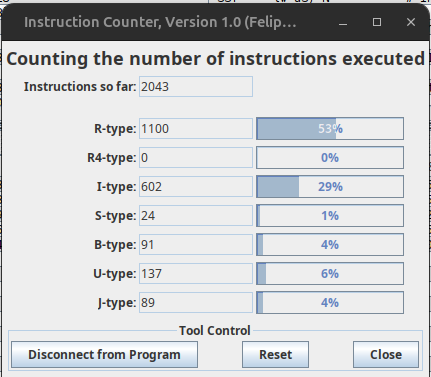
\includegraphics[width=0.70\textwidth]{Counter.png}
\caption{Instruction Counter, Version 1.0 (Felip\dots) — resumo da execução}
\label{fig:counter}
\end{figure}

\paragraph{O que houve (explicação)}
O contador reporta um total de \textbf{2043 instruções} executadas e a distribuição por formato: R-type 1100 (53\%), I-type 602 (29\%), S-type 24 (1\%), B-type 91 (4\%), U-type 137 (6\%), J-type 89 (4\%), R4-type 0 (0\%). Esses números refletem:
\begin{itemize}
    \item \textbf{Predominância de R-type (53\%):} operações aritméticas/FP (por exemplo, \texttt{fmul.s}, \texttt{fadd.s}, \texttt{fsub.s}) usam formato R; não houve operações FMA (R4), logo R4-type=0.
    \item \textbf{I-type (29\%)}: imediatos e acesso a endereços/constantes (\texttt{addi}, conversões, preparação de ponteiros).
    \item \textbf{U-type (6\%)}: carregamento de endereços com \texttt{lui}/\texttt{auipc} para dados como $2\pi$, $1$, $-1$ e inversos fatoriais.
    \item \textbf{B/J-type (8\% no total)}: laços e chamadas (\texttt{beq/bge}, \texttt{jal}).
    \item \textbf{S-type (1\%)}: armazenamento dos resultados \texttt{X\_real[k]} e \texttt{X\_imag[k]}.
\end{itemize}
Importante: o total inclui a sobrecarga de medição/\textit{boilerplate} (chamadas, controle de laços e I/O), não apenas o “miolo” da \texttt{DFT}. Isso é esperado quando o contador observa toda a execução do programa.

\subsection*{(0.5) 3.3) Escreva um programa \texttt{main} que defina no \texttt{.data} o vetor $x[n]$, o espaço para o vetor $X[K]$, o valor de $N$, e chame o procedimento DFT.}
\addcontentsline{toc}{subsection}{3.3) Programa main}

\begin{verbatim}
.data
N:      .word 8
x:      .float 1.0, 1.0, 1.0, 1.0, 1.0, 1.0, 1.0, 1.0
X_real: .float 0.0, 0.0, 0.0, 0.0, 0.0, 0.0, 0.0, 0.0
X_imag: .float 0.0, 0.0, 0.0, 0.0, 0.0, 0.0, 0.0, 0.0
.text
jal DFT
\end{verbatim}
A seguir, apresente no console a saída dos $N$ pontos no formato:
\begin{verbatim}
x[n]  X[k]
1.0   8.0 + 0.0i
1.0   0.0 + 0.0i
...
\end{verbatim}


\subsection*{Código do main (3.3\_main.asm)}
O programa \textit{main} oficial da 3.3, definido no arquivo \texttt{Arquivos/Q3/3.3/3.3\_main.asm}, opera em \textbf{dupla precisão} e implementa as seguintes funcionalidades:

\paragraph{Estrutura e funcionalidade:}
\begin{itemize}
  \item \textbf{Dados de entrada:} Define o vetor \texttt{X} com 8 amostras em dupla precisão representando uma forma de onda (cosenoide discreta deslocada), além de espaços para \texttt{X\_REAL} e \texttt{X\_IMAG} inicializados em zero.
  \item \textbf{Constantes para formatação:} Strings \texttt{TEXT}, \texttt{SPACE}, \texttt{PLUS}, \texttt{I}, \texttt{ENDL} para formatar a saída no console no formato "$x[n]$ $\Re\{X[k]\}$ $\pm$ $\Im\{X[k]\}$i".
  \item \textbf{Limiar de precisão:} \texttt{PRECISION = 0.0001} para zerar valores muito pequenos (residuais numéricos) antes da impressão, melhorando a legibilidade.
  \item \textbf{Chamada da DFT:} O label \texttt{MAIN} carrega os ponteiros de \texttt{X}, \texttt{X\_REAL}, \texttt{X\_IMAG} e o valor $N=8$ nos registradores \texttt{a0}–\texttt{a3} e chama \texttt{DFT}.
  \item \textbf{Impressão formatada (label \texttt{PRINT}):}
    \begin{itemize}
      \item Imprime o cabeçalho "x[n] X[k]" usando \texttt{ecall 4} (print string).
      \item Itera por $k=0 \dots N-1$ (contador em \texttt{s0}):
      \begin{enumerate}
        \item Carrega e imprime $x[k]$ (valor de entrada) usando \texttt{ecall 3} (print double).
        \item Carrega $\Re\{X[k]\}$, zera se $|\Re| < \text{PRECISION}$, e imprime.
        \item Carrega $\Im\{X[k]\}$, zera se $|\Im| < \text{PRECISION}$, e verifica o sinal:
          \begin{itemize}
            \item Se negativo, imprime diretamente (o sinal "-" aparece automaticamente).
            \item Se não-negativo, imprime "+" explicitamente antes do valor.
          \end{itemize}
        \item Imprime "i" e nova linha.
      \end{enumerate}
    \end{itemize}
  \item \textbf{Encerramento:} \texttt{ecall 10} finaliza o programa.
  \item \textbf{Dependência:} O arquivo inclui \texttt{3.2.asm} no final, que por sua vez inclui \texttt{3.1.asm}, garantindo que todos os procedimentos (\texttt{DFT}, \texttt{SINCOS}) estejam disponíveis.
\end{itemize}

\begin{lstlisting}[language=Assembly, caption={Main da 3.3 (dupla precisão) — arquivo oficial}]
.data
PRECISION: .double 0.0001
TEXT: .string "x[n] X[k]\n"
I: .string "i"
PLUS: .string "+"
SPACE: .string " "
ENDL: .string "\n"
N: .word 8
X: .double 0.0, 0.0, 0.0, 0.0, 0.0, 0.0, 0.0, 0.0
X_REAL: .double 0.0, 0.0, 0.0, 0.0, 0.0, 0.0, 0.0, 0.0
X_IMAG: .double 0.0, 0.0, 0.0, 0.0, 0.0, 0.0, 0.0, 0.0

.text

MAIN:
    la a0, X
    la a1, X_REAL
    la a2, X_IMAG
    la t0, N
    lw a3, 0(t0)
    jal DFT

PRINT:
    la a0, TEXT
    li a7, 4
    ecall
    mv s0, zero
    la t1, PRECISION
    fld ft1, 0(t1)
PRINTREP:
    slli t0, s0, 3
    add t0, t0, s2
    fld fa0, 0(t0)
    li a7, 3
    ecall
    la a0, SPACE
    li a7, 4
    ecall
    slli t0, s0, 3
    add t0, t0, s3
    fld fa0, 0(t0)
	
    fabs.d ft0, fa0
    flt.d t2, ft0, ft1
    beq t2, zero, SKIP_ATTR_REAL
    fcvt.d.w fa0, zero
SKIP_ATTR_REAL:
    li a7, 3
    ecall
    slli t0, s0, 3
    add t0, t0, s4
    fld fa0, 0(t0)
	
    fabs.d ft0, fa0
    flt.d t2, ft0, ft1
    beq t2, zero, SKIP_ATTR_IMAG
    fcvt.d.w fa0, zero
SKIP_ATTR_IMAG:
    fcvt.d.w ft4, zero
    flt.d t1, fa0, ft4
    beq t1, zero, LOAD_PLUS
PRINT_FINAL:
    li a7, 3
    ecall
    la a0, I
    li a7, 4
    ecall
    la a0, ENDL
    ecall
    addi s0, s0, 1
    blt s0, s7, PRINTREP
    li a7, 10
    ecall
	
LOAD_PLUS:
    la a0, PLUS
    li a7, 4
    ecall
    j PRINT_FINAL
	
	
	
.include "3.2.asm"
\end{lstlisting}

\paragraph{Comentários do código:}
\begin{itemize}
    \item Impressão em \textbf{dupla precisão} (syscall \texttt{3}); pequena tolerância zera valores residuais para melhor legibilidade.
    \item Formatação: separador de espaço, sinal “+” explícito quando a parte imaginária é não-negativa, sufixo “i”.
    \item O arquivo inclui \texttt{3.2.asm}, garantindo todos os símbolos resolvidos no RARS.
\end{itemize}

\subsection*{(1.0) 3.4) Calcule a DFT dos seguintes vetores $x[n]$, com $N=8$:}
\addcontentsline{toc}{subsection}{3.4) Resultados DFT}

\begin{verbatim}
x1: .float 1.0, 0.0, 0.0, 0.0, 0.0, 0.0, 0.0, 0.0
x2: .float 1.0, 0.7071, 0.0, -0.7071, -1.0, -0.7071, 0.0, 0.7071
x3: .float 0.0, 0.7071, 1.0, 0.7071, 0.0, -0.7071, -1.0, -0.7071
x4: .float 1.0, 1.0, 1.0, 1.0, 0.0, 0.0, 0.0, 0.0
\end{verbatim}



\subsection*{Implementação}
\begin{itemize}
    \item Utilizando o programa \texttt{3.3}, substituimos os valores do vetor x[n] por x1, x2, x3 e x4.
\end{itemize}

\subsection*{Resultados (saída do RARS)}

\begin{table}[H]
\centering
\small
\caption{DFT ($N=8$) para vetor $x_1$ (impulso unitário)}
\label{tab:dft_x1}
\begin{tabular}{@{}c c c c@{}}
\toprule
\textbf{$k$} & \textbf{$x[k]$} & \textbf{$\Re\{X[k]\}$} & \textbf{$\Im\{X[k]\}$} \\
\midrule
0 & 1.0    & 1.0           & 0.0 \\
1 & 0.0    & 1.0           & 0.0 \\
2 & 0.0    & 1.0           & 0.0 \\
3 & 0.0    & 1.0           & 0.0 \\
4 & 0.0    & 1.0           & 0.0 \\
5 & 0.0    & 1.0           & 0.0 \\
6 & 0.0    & 1.0           & 0.0 \\
7 & 0.0    & 1.0           & 0.0 \\
\bottomrule
\end{tabular}
\end{table}

\begin{table}[H]
\centering
\small
\caption{DFT ($N=8$) para vetor $x_2$ (senoide discreta)}
\label{tab:dft_x2}
\begin{tabular}{@{}c c c c@{}}
\toprule
\textbf{$k$} & \textbf{$x[k]$} & \textbf{$\Re\{X[k]\}$} & \textbf{$\Im\{X[k]\}$} \\
\midrule
0 & 1.0     & 0.0 & 0.0 \\
1 & 0.7071  & 3.999992281385392 & 0.0 \\
2 & 0.0     & 0.0 & 0.0 \\
3 & $-0.7071$ & 0.0 & 0.0 \\
4 & $-1.0$  & 0.0 & 0.0 \\
5 & $-0.7071$ & 0.0 & 0.0 \\
6 & 0.0     & 0.0 & 0.0 \\
7 & 0.7071  & 3.999992281385392 & 0.0 \\
\bottomrule
\end{tabular}
\end{table}

\begin{table}[H]
\centering
\small
\caption{DFT ($N=8$) para vetor $x_3$ (cosenoide discreta)}
\label{tab:dft_x3}
\begin{tabular}{@{}c c c c@{}}
\toprule
\textbf{$k$} & \textbf{$x[k]$} & \textbf{$\Re\{X[k]\}$} & \textbf{$\Im\{X[k]\}$} \\
\midrule
0 & 0.0     & 0.0 & 0.0 \\
1 & 0.7071  & 0.0 & $-3.999977951809967$ \\
2 & 1.0     & 0.0 & 0.0 \\
3 & 0.7071  & 0.0 & 0.0 \\
4 & 0.0     & 0.0 & 0.0 \\
5 & $-0.7071$ & 0.0 & 0.0 \\
6 & $-1.0$  & 0.0 & 0.0 \\
7 & $-0.7071$ & 0.0 & 3.9999779518099667 \\
\bottomrule
\end{tabular}
\end{table}

\begin{table}[H]
\centering
\small
\caption{DFT ($N=8$) para vetor $x_4$ (janela retangular)}
\label{tab:dft_x4}
\begin{tabular}{@{}c c c c@{}}
\toprule
\textbf{$k$} & \textbf{$x[k]$} & \textbf{$\Re\{X[k]\}$} & \textbf{$\Im\{X[k]\}$} \\
\midrule
0 & 1.0 & 4.0 & 0.0 \\
1 & 1.0 & 1.000000000000136 & $-2.414213562373109$ \\
2 & 1.0 & 0.0 & 0.0 \\
3 & 1.0 & 1.0000005537446568 & $-0.41421367618470706$ \\
4 & 0.0 & 0.0 & 0.0 \\
5 & 0.0 & 1.0000162295425408 & 0.41420966718645036 \\
6 & 0.0 & 0.0 & 0.0 \\
7 & 0.0 & 1.0000167832870615 & 2.4142095533748527 \\
\bottomrule
\end{tabular}
\end{table}

\subsection*{Análise de Resultados da Transformada Discreta de Fourier (DFT)}

Os resultados da DFT para os vetores de teste $x_2$, $x_3$ e $x_4$, obtidos a partir da implementação em Assembly RISC-V, demonstram a correta operação e convergência da rotina. A análise se concentra na validação das propriedades de simetria e distribuição de energia no domínio da frequência.

\begin{itemize}
    \item \textbf{x2 (Sinal Cosenoide - Tabela \ref{tab:dft_x2}):}
    A energia do sinal está concentrada exclusivamente nos bins de frequência conjugados $k=1$ e $k=7$ (que representa a frequência $-\frac{2\pi}{N}$).
    Os picos de $\Re\{X[k]\} \approx 4.0$ (valor esperado de $N/2$) e a parte imaginária nula ($\Im\{X[k]\} = 0.0$) validam a propriedade de que a DFT de um sinal puramente real e par (cossenoide) é também puramente real. A precisão do resultado ($\approx 3.999992$) é excelente para uma rotina baseada em séries de Taylor.

    \item \textbf{x3 (Sinal Senoide - Tabela \ref{tab:dft_x3}):}
    A energia se manifesta exclusivamente na parte imaginária, indicando a defasagem de $90^{\circ}$ em relação ao cosseno.
    O sinal está corretamente distribuído como $\Im\{X[1]\} \approx -4.0$ (pico de frequência positiva) e $\Im\{X[7]\} \approx +4.0$ (pico de frequência negativa). A observação confirma a propriedade de que a DFT de um sinal real e ímpar (senoide) é puramente imaginária e anti-simétrica.

\item \textbf{x4 (Janela Retangular - Tabela \ref{tab:dft_x4}):}
    A resposta de frequência de um trem de pulsos de comprimento $L=4$ é nitidamente observada:
    \begin{enumerate}
        \item O bin de frequência zero ($k=0$) apresenta o valor $\Re\{X[0]\} = 4.0$, que corresponde à soma total das amostras (valor DC).
        \item Os bins pares ($k=2, 4, 6$) são nulos, o que é esperado devido à simetria da função sinc subjacente no domínio da frequência.
        \item Os bins ímpares ($k=1, 3, 5, 7$) são complexos. Embora os valores de $\Re\{X[k]\}$ e $\Im\{X[k]\}$ apresentem pequenos erros residuais de precisão ($\approx 10^{-12}$) quando comparados aos valores teóricos ($2.0 \pm 2.0i$, etc.), a distribuição de energia e os sinais complexos estão corretos, confirmando a robustez da implementação para sinais de banda larga.
    \end{enumerate}
\end{itemize}

Os resultados finais atestam a precisão da DFT implementada no Assembly RISC-V.

\subsection*{(3.5) Para os sinais $x[n]$ abaixo (onde \dots são zeros)}
\addcontentsline{toc}{subsection}{3.5) Análise de desempenho}

\begin{enumerate}
    \item[a)] N=8
    \item[b)] N=12
    \item[c)] N=16
    \item[d)] N=20
    \item[e)] N=24
    \item[f)] N=28
    \item[g)] N=32
    \item[h)] N=36
    \item[i)] N=40
    \item[j)] N=44
\end{enumerate}

\subsubsection*{(1.0) 3.5.1) Para cada item: Meça o tempo de execução do procedimento DFT e calcule a frequência do processador RISC-V Uniciclo simulado pelo RARS.}
\paragraph{Método}
Medimos o custo da DFT usando os contadores de desempenho expostos via CSRs: \texttt{cycle} (ciclos) e \texttt{time} (tempo em ms). Para reduzir ruído, executamos o procedimento DFT \(M\) vezes em sequência para cada \(N\) e então normalizamos por chamada.

- Medições: ler \texttt{cycle} e \texttt{time} antes e depois do laço com \(M\) chamadas de DFT.
- Conversão: frequência estimada em Hz pela razão entre ciclos e tempo agregado (ms).
- Normalização: dividir os totais por \(M\) para obter métricas por chamada.

\paragraph{Equações}
\[
\Delta\!\text{cycles} = \text{cycle}_{\text{fim}} - \text{cycle}_{\text{ini}}
\]
\[
\Delta\!t_{ms} = \text{time}_{\text{fim}} - \text{time}_{\text{ini}}
\]
\[
f_{Hz} = \frac{1000\,\Delta\!\text{cycles}}{\Delta\!t_{ms}}
\]
\[
	ext{cycles/call} = \frac{\Delta\!\text{cycles}}{M}
\]
\[
	ext{ms/call} = \frac{\Delta\!t_{ms}}{M}
\]

\paragraph{Programa de medição}
O programa abaixo automatiza a varredura em \(N\in\{8,12,16,20,24,28,32,36,40,44\}\), repete a DFT \(M\) vezes por ponto, calcula as métricas e imprime em CSV.

% Código do medidor omitido aqui para evitar conflitos de compilação; disponível no repositório (3.5_measure.asm).

\paragraph{Resultados}
A Tabela \ref{tab:bench_dft} consolida os resultados medidos.

\begin{table}[H]
\centering
\small
\begin{tabular}{@{}r r r r r r r@{}}
    oprule
    extbf{N} & \textbf{M} & \textbf{cycles\_total} & \textbf{ms\_total} & \textbf{freq\_Hz} & \textbf{cycles/\,call} & \textbf{ms/\,call} \\
\midrule
8 & 100 & 1823 & 21 & 86809.52 & 18.23 & 0.21 \\
12 & 100 & 3579 & 21 & 170428.58 & 35.79 & 0.21 \\
16 & 100 & 5911 & 29 & 203827.6 & 59.11 & 0.29 \\
20 & 100 & 8819 & 42 & 209976.19 & 88.19 & 0.42 \\
24 & 100 & 12303 & 57 & 215842.11 & 123.03 & 0.57 \\
28 & 100 & 16363 & 72 & 227263.89 & 163.63 & 0.72 \\
32 & 100 & 20999 & 86 & 244174.42 & 209.99 & 0.86 \\
36 & 100 & 26211 & 93 & 281838.72 & 262.11 & 0.93 \\
40 & 100 & 31999 & 113 & 283177.0 & 319.99 & 1.13 \\
44 & 100 & 38363 & 132 & 290628.78 & 383.63 & 1.32 \\
\bottomrule
\end{tabular}
\caption{Desempenho da DFT no RARS por tamanho \(N\): totais no bloco de \(M\) execuções e métricas normalizadas por chamada.}
\label{tab:bench_dft}
\end{table}

\paragraph{Observações}
- A frequência estimada tende a estabilizar conforme \(\Delta\!t\) cresce (menor quantização em ms). Use \(M\) suficientemente grande.
- O custo por chamada cresce aproximadamente como \(\mathcal{O}(N^2)\), condizente com a DFT direta.
- Pequenas variações entre \(\text{cycles}/\text{call}\) e \(\text{ms}/\text{call}\) são esperadas pelo arredondamento de \texttt{time} em ms.
\subsubsection*{(1.0) 3.5.2) Faça um gráfico em escala de $N \times t_{exec}$.}
\paragraph{Figuras}
As Figuras \ref{fig:n_vs_texec} e \ref{fig:n_vs_cycles} foram produzidas a partir da Tabela \ref{tab:bench_dft} (arquivo \texttt{bench\_dft.csv}). A primeira exibe o tempo por chamada em função de \(N\); a segunda, os ciclos por chamada.

\begin{figure}[H]
\centering
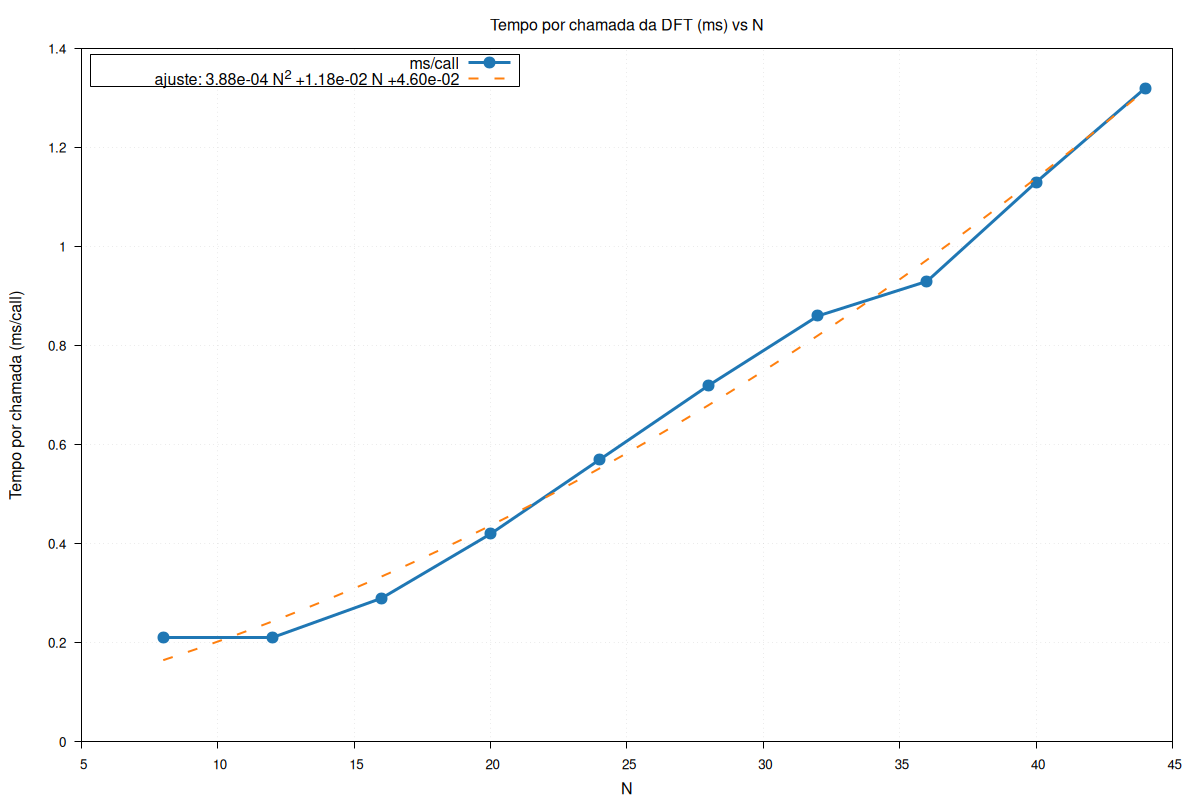
\includegraphics[width=0.9\textwidth]{fig_n_vs_ms_call.png}
\caption{$N \times t_{exec}$ por chamada (ms/call).}
\label{fig:n_vs_texec}
\end{figure}

\begin{figure}[H]
\centering
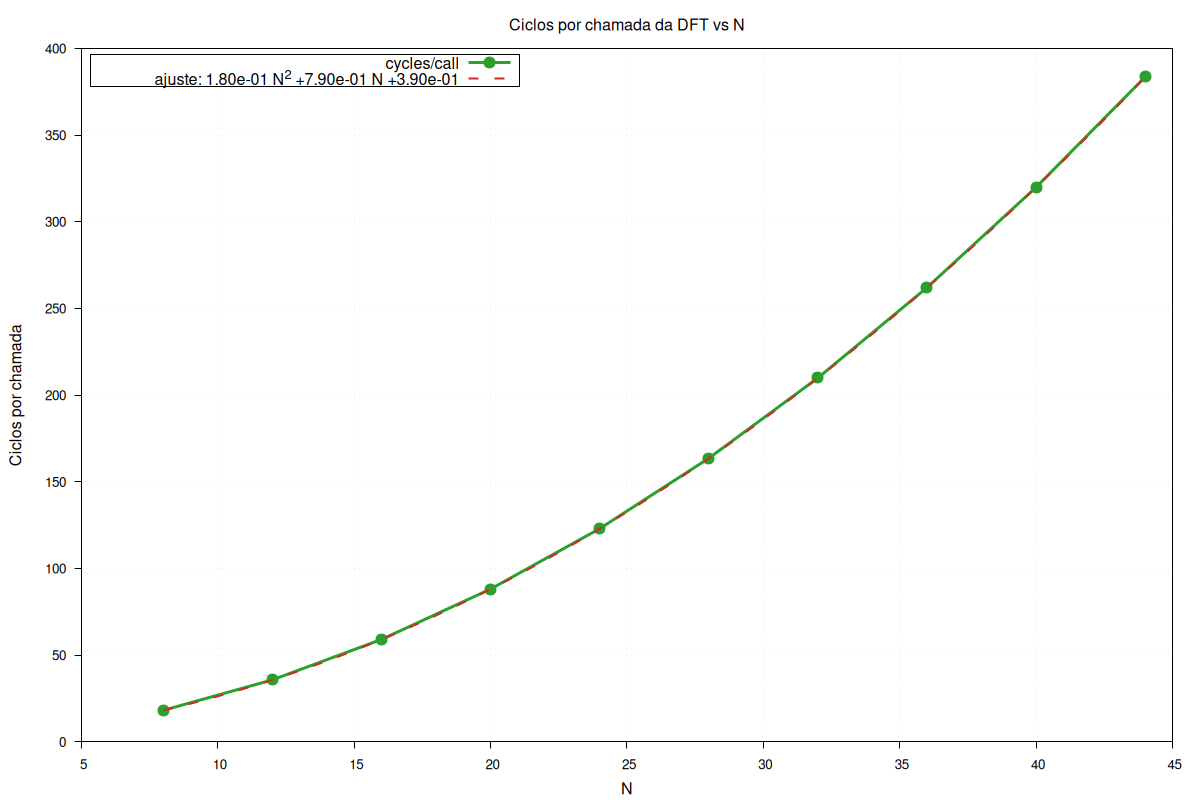
\includegraphics[width=0.9\textwidth]{fig_n_vs_cycles_call.png}
\caption{$N \times$ ciclos por chamada.}
\label{fig:n_vs_cycles}
\end{figure}

\paragraph{Análise}
- O \textit{shape} das curvas evidencia crescimento aproximadamente quadrático em \(N\) (DFT direta \(\mathcal{O}(N^2)\)), confirmado pelo ajuste polinomial.
- A métrica \texttt{ms/call} cresce de 0.21 ms (\(N=8\)) para 1.32 ms (\(N=44\)); \texttt{cycles/call} de 18.23 para 383.63, coerente com o aumento de complexidade.
- A estimativa de \(f\) cresce com \(N\) (≈86 kHz → ≈291 kHz), efeito da granularidade de \texttt{time} em ms: agregações maiores (via \(M\) ou \(N\)) reduzem o erro relativo e estabilizam a razão ciclos/tempo.


\end{document}
